\documentclass[twocolumn]{article}

\usepackage[margin=0.5in]{geometry}

\usepackage{amsmath}
\usepackage{commath}
\usepackage{graphicx}
\usepackage{hyperref}
\usepackage{enumitem}
\usepackage{mathtools}
\usepackage{flushend}

\title{1.5 Notes}
\author{}
\date{}

\begin{document}
    \maketitle

    \section*{Key Concepts}
    \subsection*{Arithmetic Sequences}
    An \textbf{arithmetic sequence}, also known as an \textbf{arithmetic
    progression}, is a sequence of numbers where the difference between
    consecutive terms are equal. For example, $2, 5, 8, 11, \dots$ is an
    arithmetic sequence because each term is $3$ more than the term before
    it. The difference between consecutive terms in an arithmetic sequence
    is called the \textbf{common difference}. If this difference is
    negative, than the sequence is decreasing. To get from one term to the
    next, we add the common difference. To get from one term to the previous
    term, we subtract the common difference.

    To find the terms of an arithmetic sequence, we can use the formula
    \[a_n = a_m + (n - m)d\] $a_n$ is the $n$th term, $a_m$ is the $m$th
    term, and $d$ is the common difference. You should be able to see how
    this formula corresponds to the definition above. To get from the $m$th
    term to the $n$th term, we need to add the common difference $n - m$
    times. We can use this formula so solve problems involving the terms of
    arithmetic sequences. For example, if we know that the second term of a
    sequence is $3$ and the common difference is $2$, the fifth term would
    be $3 + (5 - 2)2 = 9$. We can also solve for the value of $d$ if we know
    two of the terms.

    \subsection*{Arithmetic Series}
    A \textbf{series} is just the sum of the terms of a sequence. $2, 5, 8,
    11$ is an arithmetic sequence, so $2 + 5 + 8 + 11$ is an arithmetic
    series. We can find the sum of an arithmetic series by computing each
    term of the sequence and adding them all up, but that can take a long
    time when there are a large number of terms. It turns out that there is
    a simple formula that can be used to find the sum of an arithmetic
    series:
    \[S = \frac{n(a_1 + a_n)}{2}\] $S$ is the sum of the arithmetic series
    starting with $a_1$ and ending with $a_n$, or $a_1 + a_2 + \dots + a_n$.
    $n$ is the number of terms. We can prove this formula by first writing
    the arithmetic series in two different ways:
    \begin{align*}
        S &= \begin{multlined}[t]
            a_1 + (a_1 + d) + (a_1 + 2d) + \dots \\
            + (a_1 + (n - 2)d) + a_1 + (n - 1)d)
        \end{multlined} \\
        S &= \begin{multlined}[t]
            a_n + (a_n - d) + (a_n - 2d) + \dots \\
            + (a_n - (n - 2)d) + (a_n - (n - 1)d)
        \end{multlined}
    \end{align*}
    In the first way, we start with the first term and then repeatedly add
    $d$ to obtain successive terms until we reach last term. In the second
    way, we start with the last term and then repeatedly subtract $d$ to
    obtain successive terms until we reach the first term. If we add these
    two together, all the $d$ values cancel out and we get $2S = n(a_1 +
    a_n)$, which means $S = \frac{n(a_1 + a_n)}{2}$.

    We can also substitute $a_n = a_1 + (n - 1)d$ to get a formula for the
    sum in terms of $a_1$, $n$, and $d$:
    \[S = na_1 + \frac{n(n - 1)}{2}d\]

    The formula for the sum of an arithmetic series leads us to some useful
    properties of arithmetic sequences.  The mean of an arithmetic sequence
    is its sum divided by the number of terms, which is $\frac{S}{n}$.
    Looking at the first formula for the sum of an arithmetic series, we see
    that this is equal to $\frac{a_1 + a_n}{2}$. Therefore, the mean of an
    arithmetic sequence is equal to the mean of the first and last terms. If
    we substitute $a_n = a_1 + (n - 1)d$ into $\frac{a_1 + a_n}{2}$, we get
    $\frac{2a_1 + (n - 1)d}{2} = a_2 + \frac{n - 1}{2}d$. If there are an
    odd number of terms, this is equal to the term in the middle of the
    sequence. If there are an even number of terms, this is equal to the
    mean of the two terms in the middle. Therefore, the mean of an
    arithmetic sequence is equal to its median.

    The sums of a arithmetic series which start with $1$ and have common
    difference $1$ are called \textbf{triangular numbers}. Some examples are
    $1 + 2 + 3 = 6$ and $1 + 2 + 3 + 4 + 5 = 15$. These numbers are called
    triangular numbers because the $n$th triangular number is the number of
    dots needed to form an triangle pattern of size $n$:
    \begin{center}
        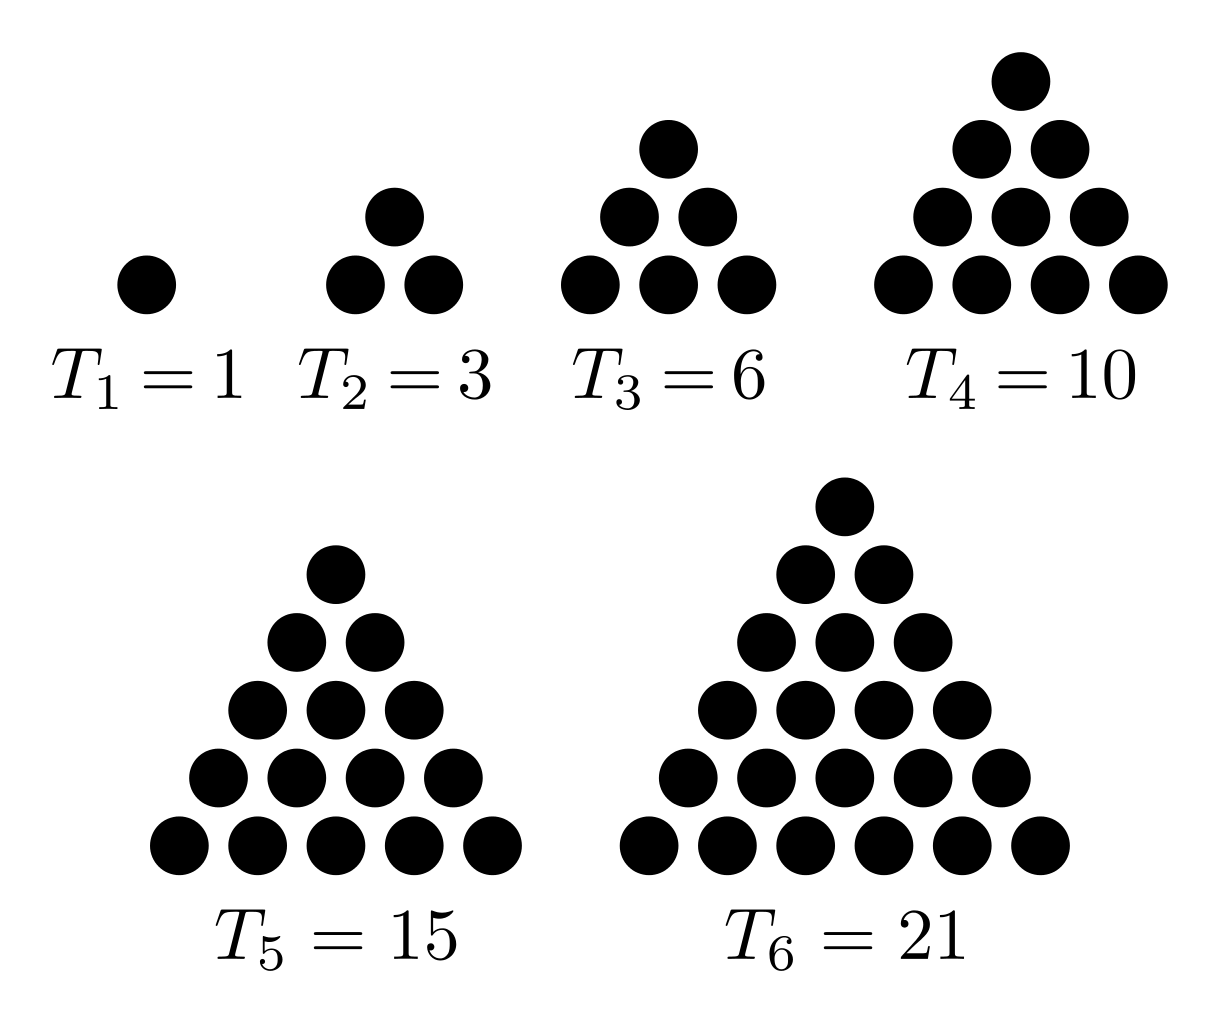
\includegraphics[width=6cm]{triangular_numbers}

        By Melchoir - Own work, CC BY-SA 3.0,
        \url{https://commons.wikimedia.org/w/index.php?curid=16942149}
    \end{center}
    We can also define the $n$th triangular number as the sum of the first
    $n$ positive integers. The formula for triangular numbers is
    \[T_n = \frac{n(n + 1)}{2}\] which is just a special case of the
    arithmetic series sum formula.

    \subsection*{Geometric Sequences}
    A \textbf{geometric sequence} is like an arithmetic sequence, except
    that the ratio between consecutive terms is constant instead of the
    difference. This ratio is called the \textbf{common ratio}. For example,
    $3, 6, 12, 24, \dots$ is a geometric sequence. To get from one term to
    the next, we multiply by the common ratio. To get from one term to the
    previous term, we divide by the common ratio.

    The formula for the terms of a geometric sequence is
    \[a_n = a_mr^{n - m}\] $a_n$ is the $n$th term, $a_m$ is the $m$th term,
    and $r$ is the common ratio.

    \subsection*{Geometric Series}
    To find the sum of a geometric series, we can use the formula
    \[S = a_1 \frac{1 - r^n}{1 - r}\] Here's the proof of the above formula:
    \begin{align*}
        S &= a_1 + a_2 + \dots + a_n \\
        Sr &= a_1 r + a_2 r + \dots + a_n r \\
        Sr &= a_2 + a_3 + \dots + a_{n + 1} \\
        S - Sr &= a_1 - a_{n + 1} \\
        S(1 - r) &= a_1 - a_{n + 1} \\
        S &= \frac{a_1 - a_{n + 1}}{1 - r} \\
        S &= \frac{a_1 - a_1 r^n}{1 - r} \\
        S &= a_1 \frac{1 - r^n}{1 - r}
    \end{align*}

    So far, we've only looked at series with finite numbers of terms. But it
    turns out that a geometric series which goes on forever can actually
    have a finite sum. For example, consider $1 + \frac{1}{2} + \frac{1}{4}
    + \frac{1}{8} + \dots$. This is a geometric series with common ratio
    $\frac{1}{2}$. If you computed $1 + \frac{1}{2}$, $1 + \frac{1}{2} +
    \frac{1}{4}$, $1 + \frac{1}{2} + \frac{1}{4} + \frac{1}{8}$, and so on,
    you will notice that these sums get closer and closer to $2$. We say
    that the sum of this infinite geometric series is equal to $2$ since as
    we add on more terms the sum gets infinitely closer to $2$. The formula
    for the sum of an infinite geometric series is quite simple:
    \[S = \frac{a_1}{1 - r}\] Here's the proof, which is similar to proof
    for the finite geometric series sum formula:
    \begin{align*}
        S &= a_1 + a_2 + a_3 + \dots \\
        Sr &= a_1 r + a_2 r + a_3 r + \dots \\
        Sr &= a_2 + a_3 + a_4 + \dots \\
        S - Sr &= a_1 \\
        S(1 - r) &= a_1 \\
        S &= \frac{a_1}{1 - r}
    \end{align*}
    Not all infinite geometric series have finite sums. The series $1 + 2 +
    4 + 8 + \dots$ clearly grows infinitely. We say that the series
    \textbf{converges} if it has a finite sum and we say that it
    \textbf{diverges} otherwise. An infinite geometric series with common
    ratio $r$ has a finite sum if and only if $\abs{r} < 1$. To see why,
    consider what happens to the finite geometric series sum as we increase
    $n$. If $\abs{r} < 1$, then $r^n$ will approach $0$ as $n$ gets larger
    and larger, so we end up with the infinite geometric series sum formula.

    \subsection*{Geometric Mean}
    The word ``mean'' usually refers to the \textbf{arithmetic mean}, but
    there's also something called the \textbf{geometric mean}. The geometric
    mean of the $n$ numbers $x_1, x_2, \dots, x_n$ is $\sqrt[n]{x_1 x_2
    \dots x_n}$.

    \subsection*{Inserting Means}
    ``Insert $n$ arithmetic means between $a$ and $b$'' means we need to
    insert $n$ numbers $x_1, x_2, \dots, x_n$ between $a$ and $b$ such that
    $a, x_1, x_2, \dots, x_n, b$ forms an arithmetic sequence. Similarly,
    ``insert $n$ geometric means between $a$ and $b$'' means to insert $n$
    numbers $x_1, x_2, \dots, x_n$ between $a$ and $b$ such that $a, x_1,
    x_2, \dots, x_n, b$ forms an geometric series. For example, inserting
    three arithmetic means between $1$ and $9$ results in $1, 3, 5, 7, 9$,
    and inserting two geometric means between $1$ and $8$ results in $1, 2,
    4, 8$. We can find the terms that we need to insert by using the
    arithmetic or geometric sequence formulas to find the common ratio or
    difference.

    \section*{Examples}
    \subsection*{Arithmetic Sequences}
    \begin{enumerate}
        \item A child’s mother gives her $10$ cents one day. Every day
        thereafter her mother gives her $3$ more cents than the previous
        day. After $20$ days, how much does she have?
        \vspace{3cm}
        \item Prove that
        \[a + (a + d) + (a + 2d) + \dots + (a + (n - 1)d = \frac{n}{2}(2a +
        (n - 1)d)\]
        \vspace{3cm}
        \item If the sum of the first ten terms of an arithmetic progression
        is four times the sum of the first five terms, find the ratio of the
        first term to the common difference.
        \vspace{3cm}
        \item What is the sixth term of the arithmetic sequence whose $31$st
        and $73$rd terms are $18$ and $46$, respectively?
        \vspace{3cm}
        \item Insert three arithmetic means between $3$ and $4$.
        \vspace{3cm}
    \end{enumerate}
    \subsection*{Geometric Sequences}
    \begin{enumerate}[resume]
        \item Prove that
        \[a + ar + \dots + ar^{n - 1} = \frac{a - ar^n}{1 - r}\]
        \vspace{3cm}
        \item Evaluate $2 - \frac{2}{3} + \frac{2}{9} - \frac{2}{27} +
        \frac{2}{81}$ using the finite geometric series sum formula.
        \vspace{3cm}
        \item For what value of $x$ does $1 + x + x^2 + x^3 + x^4 + \dots =
        4$?
        \vspace{3cm}
        \item Insert two geometric means between $3$ and $4$.
        \vspace{3cm}
    \end{enumerate}
\end{document}